\chapter{Introduction}
% \label{chap:intro}

% \section{Introduction}
\section{Motivations}
% \label{sec:motivation}

The process of web development has been significantly transformed by the introduction and adoption of frameworks. Frameworks have become the industry standard, providing developers with structured, reusable tools that simplify the creation of web applications. This evolution has also been greatly influenced by the rise of LLMs like OpenAI's Codex \cite{chen2021openai_codex}, Google's Gemini \cite{gemini}, and GitHub Copilot\footnote{Github Copilot - \url{https://copilot.github.com/}}, which have made coding more accessible by offering automated code generation, real-time suggestions, and debugging assistance. These tools have made entry into web development easier than ever, lowering barriers for beginners and speeding up development processes.

However, despite these advancements, LLMs still face certain limitations, such as hallucinations, difficulties in referencing external sources, and performance issues when handling specific tasks. A promising solution to mitigate these limitations is using RAG. RAG enhances the generative capabilities of LLMs by retrieving relevant external information before generating content, improving both the accuracy and relevance of the output. This technique is particularly beneficial in domains like web development, where staying up-to-date with framework versions and ensuring compatibility across services is critical. Incorporating RAG helps bridge the gap between rapidly evolving frameworks and the knowledge developers need to make informed decisions about the tools and technologies they use.

\begin{figure}[H]
\vspace{2pt}
\centering
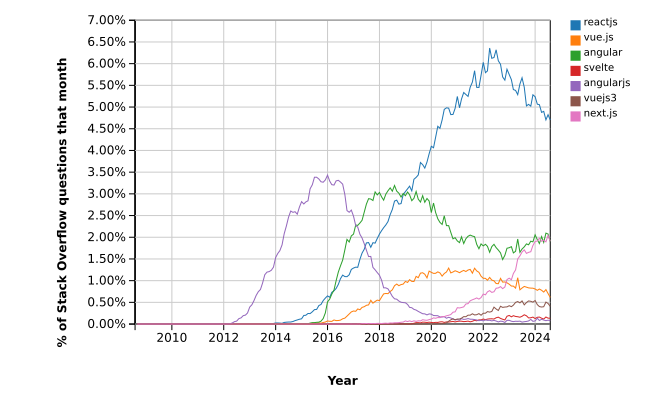
\includegraphics[width=1\textwidth]{Images/Introduction/stackoverflow-trends-chart.png}
\vspace{.1cm}
\caption{The popularity of frameworks based on StackOverflow questions 2008-2024}
\end{figure}

To illustrate, consider the Next.js framework, which exemplifies the rapid evolution of modern web technologies. Originally built on top of React.js, Next.js has transformed from a simple server-rendering tool into a comprehensive full-stack framework. What makes Next.js particularly notable is the speed at which it introduces significant updates. In just under three years, it moved from version 12 to version 15, each introducing major shifts in architecture and development paradigms.

For instance, Next.js 13 (October 2022) introduced the App Router, React Server Components, and a new file-based routing system—radically altering how pages and layouts are structured. Less than a year later, Next.js 14 (October 2023) refined these features while improving performance with deeper Turbopack integration. And most recently, Next.js 15 (March 2025) pushed the boundaries even further by stabilizing Partial Prerendering, extending Server Actions, and fully embracing React Server Components\footnote{\href{https://nextjs.org/blog/next-15}{Next.js 15 Release Notes - https://nextjs.org/blog/next-15}}.

These frequent and impactful changes challenge developers to constantly relearn patterns, adapt to breaking changes, and stay updated with both Next.js and its dependency—React.js, which itself released React 19 with major improvements to transitions, refs, and concurrency\footnote{\href{https://react.dev/blog/2024/04/25/react-19-upgrade-guide}{React 19 Upgrade Guide - https://react.dev/blog/2024/04/25/react-19-upgrade-guide}}.

\section{Problem statement}

Modern web development frameworks, such as Next.js, offer powerful features and flexibility, making them a popular choice for building high-performance applications. However, as these frameworks continue to evolve, their complexity has grown significantly. Developers are often required to refer to extensive documentation, which can be fragmented and difficult to navigate, to resolve coding challenges, learn new functionalities, or debug issues. This reliance on documentation creates several inefficiencies in the development workflow, including:

\begin{itemize}
  \item Time-Consuming Information Retrieval: Developers frequently need to search through lengthy and intricate documentation to find specific information. Traditional search methods, such as keyword-based tools, often fail to capture the intent behind the query or retrieve relevant context, leading to prolonged and unproductive searches.
  \item Fragmented Context: Even when relevant information is found, it often lacks the necessary context to answer the developer's query fully. This forces developers to cross-reference multiple sections of the documentation, further delaying progress.
  \item Disruption of Workflow: Switching between the code editor and external documentation interrupts the development process, causing a loss of focus and reducing productivity.
  \item Inconsistent Results: Existing tools, such as search engines or static code assistants, often provide inconsistent results that fail to address the specific needs of a query or task, leaving developers to piece together partial solutions on their own.
\end{itemize}


\section{Significant of the problem}

Solving this problem is of critical importance for several reasons:

\begin{itemize}
  \item Enhanced Developer Productivity: By significantly reducing the time spent searching for relevant information, the proposed system allows developers to focus on coding tasks, accelerating development timelines and increasing overall productivity.
  \item Improved Workflow Efficiency: Delivering context-aware assistance directly within the coding environment (e.g., Visual Studio Code) eliminates the need to switch between multiple tools and resources, streamlining the development process and reducing cognitive load.
  \item Support for Complex Frameworks: As frameworks like Next.js continue to evolve, the volume and complexity of their documentation will only increase. An intelligent system capable of efficiently managing and retrieving this knowledge ensures that developers can stay up-to-date and adapt to new features quickly.
\end{itemize}

By solving this problem, we aim to not only improve the efficiency of individual developers but also set a foundation for the future of Artificial Intelligent (AI), AI-assisted development environments. This research will demonstrate how advanced AI techniques like RAG can transform the way developers interact with documentation, enhancing both their productivity and their overall experience.

\section{Objectives}

The objective of this research is to develop a tool, specifically a VS Code extension, that facilitates the web development process by addressing common challenges associated with modern frameworks. The tool aims to:

\begin{itemize}
  \item Utilize RAG to assist developers with question answering, code generation, and code review. RAG will retrieve relevant information from documentation or community forums to enhance the accuracy and relevance of the tool's suggestions.
  \item Analyze the user's codebase and suggest modifications for parts that are no longer relevant, particularly when updating the code to newer versions of a framework.
\end{itemize}

This extension will help streamline the development process, making it easier for developers to maintain, upgrade, and enhance their applications with minimal friction.

\section{Scope}
The scope is intentionally confined to Next.js as the primary framework for web application development, enabling a focused exploration of its interaction with RAG methodologies. Additionally, the implementation targets applications written in JavaScript, TypeScript, HTML, and CSS, ensuring compatibility with commonly used web development programming languages.

% In this thesis, we aim to focus on the Next.js framework and the common packages that are often used alongside it, as well as Firebase for hosting purposes. The scope of the research includes the design and implementation of the RAG pipeline, the integration of the VSCode extension, and the evaluation of the system’s effectiveness in improving the development experience for Next.js applications.

% Specifically, our scope will only includes the technologies of Next.js - main framework used for the web application development.

% The tool will specifically target applications written in JavaScript, TypeScript, HTML, and CSS.
% Specifically, the scope includes the following technologies:

% \begin{itemize}
%   \item Next.js: The main framework used for web application development.
%   \item Firebase: Used for hosting Next.js applications and providing backend services.
%   \item Tailwind CSS: A utility-first CSS framework for designing responsive user interfaces.
%   \item Framer Motion: A popular library for animations and interactions.
%   \item Shadcn UI: A component library for UI elements.
%   \item Zod: A TypeScript-first schema declaration and validation library.
%   \item Prisma: An ORM for interacting with the database in a type-safe manner.
%   \item Firebase SDK: The official Firebase SDK is used for integration with Firebase services.
% \end{itemize}



% The focus will be on understanding how these tools and libraries can be used effectively in combination with Next.js and Firebase, with an emphasis on addressing issues related to rapid framework evolution and interoperability between services.

\section{Challenges}

Developing this tool involves several challenges:

\begin{itemize}
  \item Efficient context management: Since the goal is to make the tool lightweight, storing and managing the context of a user's codebase in a way that allows for fast retrieval without overwhelming system resources is a major challenge.
  \item Data curation complexity: The data curation process requires extensive knowledge about the framework.
  \item Handling framework updates: Keeping the tool updated with the frequent changes in frameworks like Next.js and their associated packages is challenging. Continuous updates are needed to ensure compatibility and provide accurate suggestions.
  \item User experience: Balancing the amount of information presented to the user without overwhelming them is essential. The tool should provide meaningful insights and recommendations without causing information overload.
\end{itemize}

\section{Structure of the report}

\textbf{Chapter 1. Introduction.} 
This chapter introduces the motivations, objectives, and scope of the research. It highlights the challenges of web development and the role of RAG in enhancing efficiency and accuracy. The chapter outlines the structure of the report, providing a roadmap for the research presented.

\textbf{Chapter 2. Preliminaries.} 
This chapter provides foundational knowledge on RAG, emphasizing its retriever and generator components. It discusses indexing, vector embeddings, and augmentation methods, offering a clear understanding of the technologies used.

\textbf{Chapter 3. Related works and tools.} 
This chapter explores prior research on RAG and its application in web development. It reviews developer tools such as VS Code extensions and discusses strategies for retrieval and augmentation. Comparative analyses of existing frameworks and methodologies are also presented.

\textbf{Chapter 4. Approach.} 
This chapter presents the reasoning behind adopting RAG over fine-tuning, and explains the selection of key components such as the BGE-M3 embedding model and Ollama's local LLMs. It also discusses design choices including containerization with Docker and the use of a VS Code extension. Finally, it outlines the system’s core architecture, focusing on local vector storage and editor integration.


\textbf{Chapter 5. Implementation.} 
This chapter details the development process of the RAGGIN system, covering data preparation, preprocessing, database design and setup, and the implementation of a RESTful API. It also introduces the core retrieval and generation services, and concludes with the integration of these components into a VS Code extension.

\textbf{Chapter 6. Evaluation.}
This chapter presents the evaluation of the system through quantitative metrics for both retrieval and generation components. It describes the evaluation methodology, summarizes results, and includes both unit and integration testing to validate system behavior. The analysis highlights key strengths as well as performance limitations under different usage scenarios.

\textbf{Chapter 7. Conclusion.}
The final chapter summarizes the key results achieved, acknowledges the current system limitations, and outlines clear directions for future development.


% Background knowledge is then provided to explain the technologies and methodologies used. A review of related work follows, including research and existing solutions in web development, and Retrieval-Augmented Generation (RAG). The approach section describes the proposed solution, detailing the architecture and methodology for building the VSCode extension. The implementation section outlines the development process, and tools used. The evaluation presents the metrics, testing strategies, and results, along with comparisons to other solutions. Finally, the conclusion summarizes the achievements, discusses limitations, and offers suggestions for future improvements, with a reference section listing all the sources used.